\documentclass[a4paper, 12pt]{article}
\usepackage{listings} 
\usepackage{xcolor}
\usepackage{mdframed}
\usepackage{graphicx}
\usepackage{pgfplots}
\usepackage{float}
\usepackage{mathtools}
\usepackage[margin=1.00in]{geometry}
\DeclarePairedDelimiter\ceil{\lceil}{\rceil}
\DeclarePairedDelimiter\floor{\lfloor}{\rfloor}

\definecolor{code-gray}{gray}{0.93}
\begin{document}
\title{ECE 440 - Project \#1}
\author{Collin Heist}
\date{\today}
\maketitle
\pagenumbering{arabic}

\section{Vivado Messages}
\begin{figure}[H]
\centering
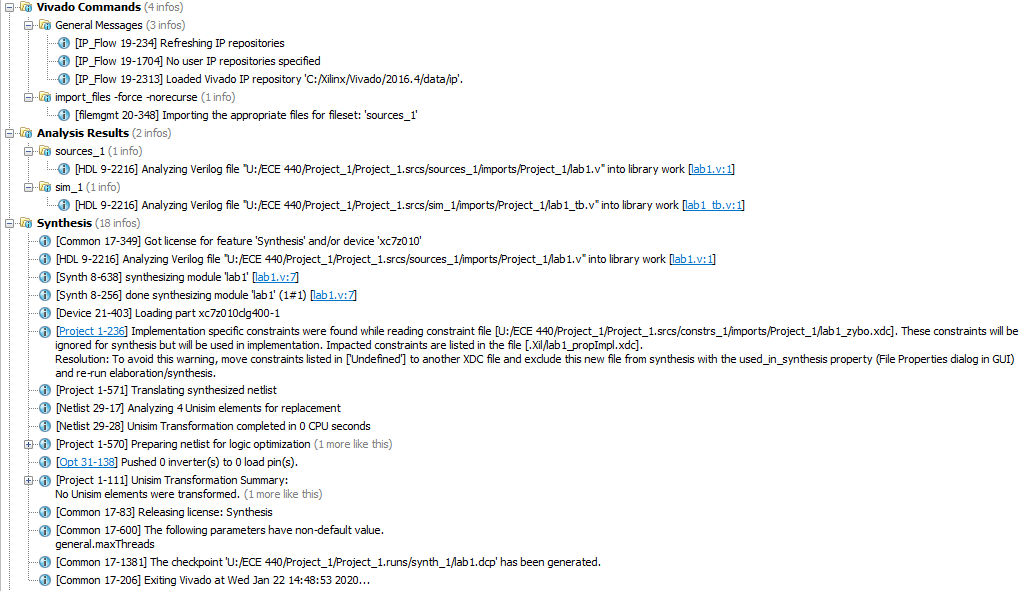
\includegraphics[width=1\textwidth]{vivado_messages1.PNG}
\caption{Screenshot 1 of the Vivado Messages screen.}
\label{fig:img00}
\end{figure}

\begin{figure}[H]
\centering
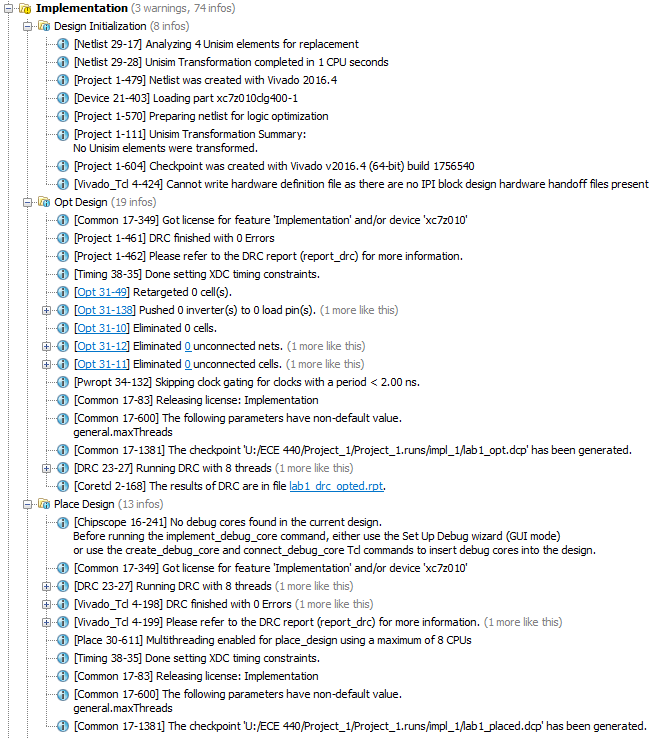
\includegraphics[width=1\textwidth]{vivado_messages2.PNG}
\caption{Screenshot 2 of the Vivado Messages screen.}
\label{fig:img00}
\end{figure}

\begin{figure}[H]
\centering
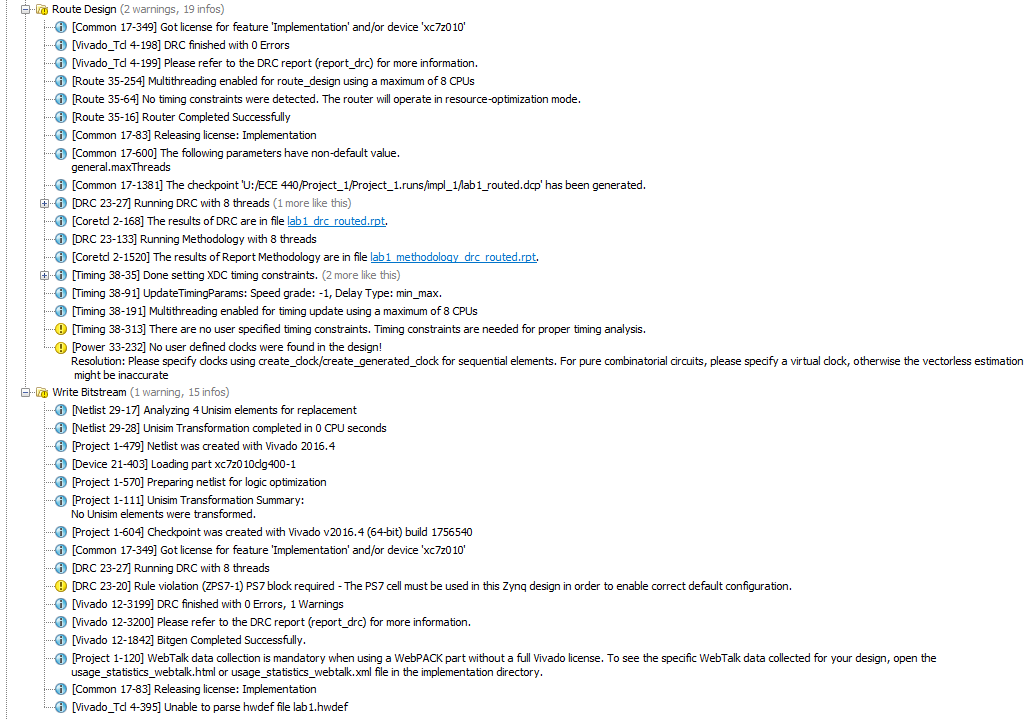
\includegraphics[width=1\textwidth]{vivado_messages3.PNG}
\caption{Screenshot 3 of the Vivado Messages screen.}
\label{fig:img00}
\end{figure}

\begin{figure}[H]
\centering
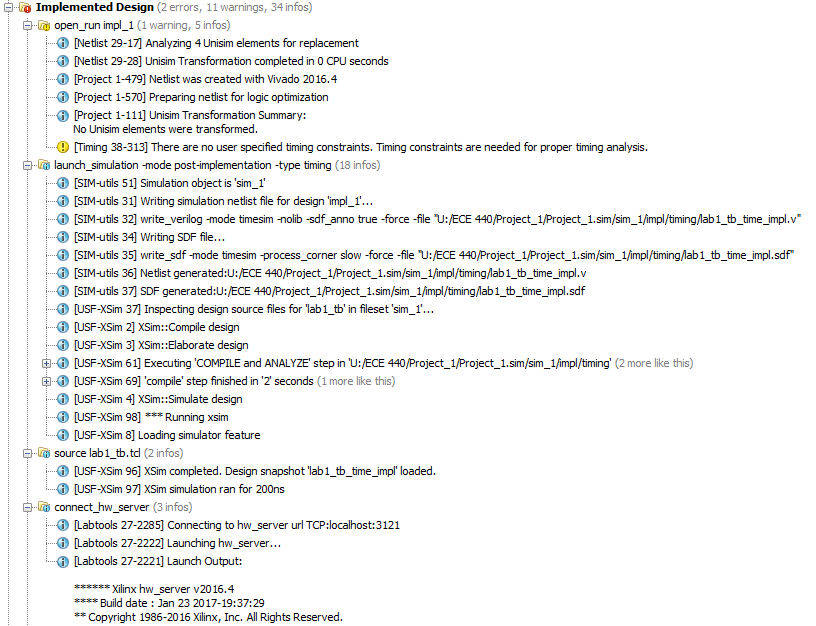
\includegraphics[width=1\textwidth]{vivado_messages4.PNG}
\caption{Screenshot 4 of the Vivado Messages screen.}
\label{fig:img00}
\end{figure}

\begin{figure}[H]
\centering
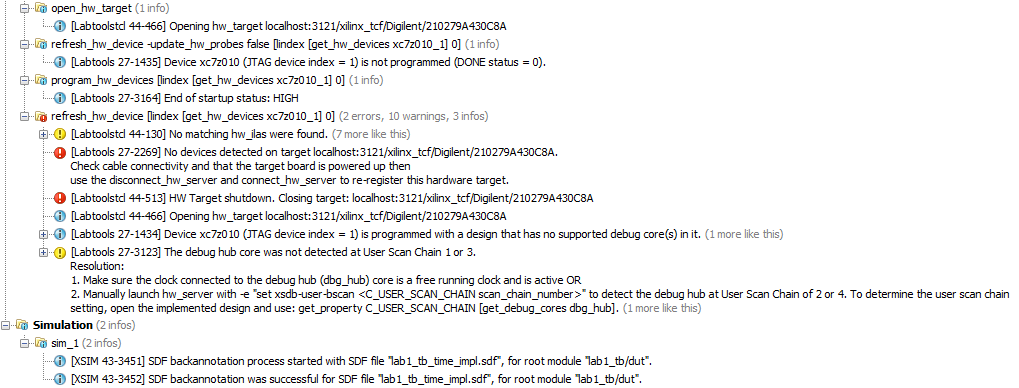
\includegraphics[width=1\textwidth]{vivado_messages5.PNG}
\caption{Screenshot 5 of the Vivado Messages screen.}
\label{fig:img00}
\end{figure}

\section{Vivado Synthesis Report}
\begin{verbatim}#-----------------------------------------------------------
# Vivado v2016.4 (64-bit)
# SW Build 1756540 on Mon Jan 23 19:11:23 MST 2017
# IP Build 1755317 on Mon Jan 23 20:30:07 MST 2017
# Start of session at: Wed Jan 22 14:48:18 2020
# Process ID: 17812
# Current directory: U:/ECE 440/Project_1/Project_1.runs/synth_1
# Command line: vivado.exe -log lab1.vds -product Vivado -mode batch -messageDb vivado.pb -notrace -source lab1.tcl
# Log file: U:/ECE 440/Project_1/Project_1.runs/synth_1/lab1.vds
# Journal file: U:/ECE 440/Project_1/Project_1.runs/synth_1\vivado.jou
#-----------------------------------------------------------
Sourcing tcl script 'C:/Xilinx/Vivado/2016.4/scripts/init.tcl'
source lab1.tcl -notrace
Command: synth_design -top lab1 -part xc7z010clg400-1
Starting synth_design
Attempting to get a license for feature 'Synthesis' and/or device 'xc7z010'
INFO: [Common 17-349] Got license for feature 'Synthesis' and/or device 'xc7z010'
INFO: Launching helper process for spawning children vivado processes
INFO: Helper process launched with PID 5396 
---------------------------------------------------------------------------------
Starting RTL Elaboration : Time (s): cpu = 00:00:05 ; elapsed = 00:00:12 . Memory (MB): peak = 325.723 ; gain = 114.543
---------------------------------------------------------------------------------
INFO: [Synth 8-638] synthesizing module 'lab1' [U:/ECE 440/Project_1/Project_1.srcs/sources_1/imports/Project_1/lab1.v:7]
INFO: [Synth 8-256] done synthesizing module 'lab1' (1#1) [U:/ECE 440/Project_1/Project_1.srcs/sources_1/imports/Project_1/lab1.v:7]
---------------------------------------------------------------------------------
Finished RTL Elaboration : Time (s): cpu = 00:00:06 ; elapsed = 00:00:12 . Memory (MB): peak = 362.977 ; gain = 151.797
---------------------------------------------------------------------------------

Report Check Netlist: 
+------+------------------+-------+---------+-------+------------------+
|      |Item              |Errors |Warnings |Status |Description       |
+------+------------------+-------+---------+-------+------------------+
|1     |multi_driven_nets |      0|        0|Passed |Multi driven nets |
+------+------------------+-------+---------+-------+------------------+
---------------------------------------------------------------------------------
Finished RTL Optimization Phase 1 : Time (s): cpu = 00:00:06 ; elapsed = 00:00:13 . Memory (MB): peak = 362.977 ; gain = 151.797
---------------------------------------------------------------------------------
INFO: [Device 21-403] Loading part xc7z010clg400-1
INFO: [Project 1-570] Preparing netlist for logic optimization

Processing XDC Constraints
Initializing timing engine
Parsing XDC File [U:/ECE 440/Project_1/Project_1.srcs/constrs_1/imports/Project_1/lab1_zybo.xdc]
Finished Parsing XDC File [U:/ECE 440/Project_1/Project_1.srcs/constrs_1/imports/Project_1/lab1_zybo.xdc]
INFO: [Project 1-236] Implementation specific constraints were found while reading constraint file [U:/ECE 440/Project_1/Project_1.srcs/constrs_1/imports/Project_1/lab1_zybo.xdc]. These constraints will be ignored for synthesis but will be used in implementation. Impacted constraints are listed in the file [.Xil/lab1_propImpl.xdc].
Resolution: To avoid this warning, move constraints listed in [.Xil/lab1_propImpl.xdc] to another XDC file and exclude this new file from synthesis with the used_in_synthesis property (File Properties dialog in GUI) and re-run elaboration/synthesis.
Completed Processing XDC Constraints

INFO: [Project 1-111] Unisim Transformation Summary:
No Unisim elements were transformed.

Constraint Validation Runtime : Time (s): cpu = 00:00:00 ; elapsed = 00:00:00.006 . Memory (MB): peak = 588.855 ; gain = 0.000
---------------------------------------------------------------------------------
Finished Constraint Validation : Time (s): cpu = 00:00:13 ; elapsed = 00:00:23 . Memory (MB): peak = 588.855 ; gain = 377.676
---------------------------------------------------------------------------------
---------------------------------------------------------------------------------
Start Loading Part and Timing Information
---------------------------------------------------------------------------------
Loading part: xc7z010clg400-1
---------------------------------------------------------------------------------
Finished Loading Part and Timing Information : Time (s): cpu = 00:00:13 ; elapsed = 00:00:23 . Memory (MB): peak = 588.855 ; gain = 377.676
---------------------------------------------------------------------------------
---------------------------------------------------------------------------------
Start Applying 'set_property' XDC Constraints
---------------------------------------------------------------------------------
---------------------------------------------------------------------------------
Finished applying 'set_property' XDC Constraints : Time (s): cpu = 00:00:13 ; elapsed = 00:00:23 . Memory (MB): peak = 588.855 ; gain = 377.676
---------------------------------------------------------------------------------
---------------------------------------------------------------------------------
Finished RTL Optimization Phase 2 : Time (s): cpu = 00:00:13 ; elapsed = 00:00:23 . Memory (MB): peak = 588.855 ; gain = 377.676
---------------------------------------------------------------------------------

Report RTL Partitions: 
+-+--------------+------------+----------+
| |RTL Partition |Replication |Instances |
+-+--------------+------------+----------+
+-+--------------+------------+----------+
---------------------------------------------------------------------------------
Start RTL Component Statistics 
---------------------------------------------------------------------------------
Detailed RTL Component Info : 
---------------------------------------------------------------------------------
Finished RTL Component Statistics 
---------------------------------------------------------------------------------
---------------------------------------------------------------------------------
Start RTL Hierarchical Component Statistics 
---------------------------------------------------------------------------------
Hierarchical RTL Component report 
---------------------------------------------------------------------------------
Finished RTL Hierarchical Component Statistics
---------------------------------------------------------------------------------
---------------------------------------------------------------------------------
Start Part Resource Summary
---------------------------------------------------------------------------------
Part Resources:
DSPs: 80 (col length:40)
BRAMs: 120 (col length: RAMB18 40 RAMB36 20)
---------------------------------------------------------------------------------
Finished Part Resource Summary
---------------------------------------------------------------------------------
---------------------------------------------------------------------------------
Start Cross Boundary and Area Optimization
---------------------------------------------------------------------------------
---------------------------------------------------------------------------------
Finished Cross Boundary and Area Optimization : Time (s): cpu = 00:00:13 ; elapsed = 00:00:23 . Memory (MB): peak = 588.855 ; gain = 377.676
---------------------------------------------------------------------------------

Report RTL Partitions: 
+-+--------------+------------+----------+
| |RTL Partition |Replication |Instances |
+-+--------------+------------+----------+
+-+--------------+------------+----------+
---------------------------------------------------------------------------------
Start Timing Optimization
---------------------------------------------------------------------------------
---------------------------------------------------------------------------------
Start Applying XDC Timing Constraints
---------------------------------------------------------------------------------
---------------------------------------------------------------------------------
Finished Applying XDC Timing Constraints : Time (s): cpu = 00:00:22 ; elapsed = 00:00:32 . Memory (MB): peak = 621.066 ; gain = 409.887
---------------------------------------------------------------------------------
---------------------------------------------------------------------------------
Finished Timing Optimization : Time (s): cpu = 00:00:22 ; elapsed = 00:00:32 . Memory (MB): peak = 621.066 ; gain = 409.887
---------------------------------------------------------------------------------

Report RTL Partitions: 
+-+--------------+------------+----------+
| |RTL Partition |Replication |Instances |
+-+--------------+------------+----------+
+-+--------------+------------+----------+
---------------------------------------------------------------------------------
Start Technology Mapping
---------------------------------------------------------------------------------
---------------------------------------------------------------------------------
Finished Technology Mapping : Time (s): cpu = 00:00:22 ; elapsed = 00:00:32 . Memory (MB): peak = 630.734 ; gain = 419.555
---------------------------------------------------------------------------------

Report RTL Partitions: 
+-+--------------+------------+----------+
| |RTL Partition |Replication |Instances |
+-+--------------+------------+----------+
+-+--------------+------------+----------+
---------------------------------------------------------------------------------
Start IO Insertion
---------------------------------------------------------------------------------
---------------------------------------------------------------------------------
Start Flattening Before IO Insertion
---------------------------------------------------------------------------------
---------------------------------------------------------------------------------
Finished Flattening Before IO Insertion
---------------------------------------------------------------------------------
---------------------------------------------------------------------------------
Start Final Netlist Cleanup
---------------------------------------------------------------------------------
---------------------------------------------------------------------------------
Finished Final Netlist Cleanup
---------------------------------------------------------------------------------
---------------------------------------------------------------------------------
Finished IO Insertion : Time (s): cpu = 00:00:22 ; elapsed = 00:00:32 . Memory (MB): peak = 630.734 ; gain = 419.555
---------------------------------------------------------------------------------

Report Check Netlist: 
+------+------------------+-------+---------+-------+------------------+
|      |Item              |Errors |Warnings |Status |Description       |
+------+------------------+-------+---------+-------+------------------+
|1     |multi_driven_nets |      0|        0|Passed |Multi driven nets |
+------+------------------+-------+---------+-------+------------------+
---------------------------------------------------------------------------------
Start Renaming Generated Instances
---------------------------------------------------------------------------------
---------------------------------------------------------------------------------
Finished Renaming Generated Instances : Time (s): cpu = 00:00:22 ; elapsed = 00:00:32 . Memory (MB): peak = 630.734 ; gain = 419.555
---------------------------------------------------------------------------------

Report RTL Partitions: 
+-+--------------+------------+----------+
| |RTL Partition |Replication |Instances |
+-+--------------+------------+----------+
+-+--------------+------------+----------+
---------------------------------------------------------------------------------
Start Rebuilding User Hierarchy
---------------------------------------------------------------------------------
---------------------------------------------------------------------------------
Finished Rebuilding User Hierarchy : Time (s): cpu = 00:00:22 ; elapsed = 00:00:32 . Memory (MB): peak = 630.734 ; gain = 419.555
---------------------------------------------------------------------------------
---------------------------------------------------------------------------------
Start Renaming Generated Ports
---------------------------------------------------------------------------------
---------------------------------------------------------------------------------
Finished Renaming Generated Ports : Time (s): cpu = 00:00:22 ; elapsed = 00:00:32 . Memory (MB): peak = 630.734 ; gain = 419.555
---------------------------------------------------------------------------------
---------------------------------------------------------------------------------
Start Handling Custom Attributes
---------------------------------------------------------------------------------
---------------------------------------------------------------------------------
Finished Handling Custom Attributes : Time (s): cpu = 00:00:22 ; elapsed = 00:00:32 . Memory (MB): peak = 630.734 ; gain = 419.555
---------------------------------------------------------------------------------
---------------------------------------------------------------------------------
Start Renaming Generated Nets
---------------------------------------------------------------------------------
---------------------------------------------------------------------------------
Finished Renaming Generated Nets : Time (s): cpu = 00:00:22 ; elapsed = 00:00:32 . Memory (MB): peak = 630.734 ; gain = 419.555
---------------------------------------------------------------------------------
---------------------------------------------------------------------------------
Start Writing Synthesis Report
---------------------------------------------------------------------------------

Report BlackBoxes: 
+-+--------------+----------+
| |BlackBox name |Instances |
+-+--------------+----------+
+-+--------------+----------+

Report Cell Usage: 
+------+-----+------+
|      |Cell |Count |
+------+-----+------+
|1     |LUT1 |     1|
|2     |LUT2 |     2|
|3     |LUT3 |     1|
|4     |IBUF |     4|
|5     |OBUF |     4|
+------+-----+------+

Report Instance Areas: 
+------+---------+-------+------+
|      |Instance |Module |Cells |
+------+---------+-------+------+
|1     |top      |       |    12|
+------+---------+-------+------+
---------------------------------------------------------------------------------
Finished Writing Synthesis Report : Time (s): cpu = 00:00:22 ; elapsed = 00:00:32 . Memory (MB): peak = 630.734 ; gain = 419.555
---------------------------------------------------------------------------------
Synthesis finished with 0 errors, 0 critical warnings and 0 warnings.
Synthesis Optimization Runtime : Time (s): cpu = 00:00:12 ; elapsed = 00:00:17 . Memory (MB): peak = 630.734 ; gain = 154.512
Synthesis Optimization Complete : Time (s): cpu = 00:00:22 ; elapsed = 00:00:32 . Memory (MB): peak = 630.734 ; gain = 419.555
INFO: [Project 1-571] Translating synthesized netlist
INFO: [Netlist 29-17] Analyzing 4 Unisim elements for replacement
INFO: [Netlist 29-28] Unisim Transformation completed in 0 CPU seconds
INFO: [Project 1-570] Preparing netlist for logic optimization
INFO: [Opt 31-138] Pushed 0 inverter(s) to 0 load pin(s).
INFO: [Project 1-111] Unisim Transformation Summary:
No Unisim elements were transformed.

INFO: [Common 17-83] Releasing license: Synthesis
15 Infos, 0 Warnings, 0 Critical Warnings and 0 Errors encountered.
synth_design completed successfully
synth_design: Time (s): cpu = 00:00:20 ; elapsed = 00:00:25 . Memory (MB): peak = 642.680 ; gain = 399.543
INFO: [Common 17-600] The following parameters have non-default value.
general.maxThreads
INFO: [Common 17-1381] The checkpoint 'U:/ECE 440/Project_1/Project_1.runs/synth_1/lab1.dcp' has been generated.
report_utilization: Time (s): cpu = 00:00:00 ; elapsed = 00:00:00.015 . Memory (MB): peak = 642.680 ; gain = 0.000
INFO: [Common 17-206] Exiting Vivado at Wed Jan 22 14:48:53 2020...
\end{verbatim}

\end{document}